\documentclass[12pt,hyperref,a4paper,UTF8]{ctexart}
\usepackage{HDUReport}
\usepackage{listings}
\usepackage{xcolor}
\usepackage{graphicx}
\usepackage{setspace}
\usepackage{subcaption}
\usepackage{float}
\setstretch{1.5} % 设置全局行距为1.5倍

\usepackage{enumitem} % 载入enumitem包以便自定义列表环境
\setlist[itemize]{itemsep=0pt, parsep=0pt} % 设置itemize环境的项目间距和段落间距

\setmainfont{Times New Roman} % 英文正文为Times New Roman


\usepackage{tikz}
\usetikzlibrary{shapes.geometric, arrows}
\usetikzlibrary{positioning, arrows.meta}
\usetikzlibrary{calc}


% 设置MATLAB代码样式
\definecolor{codegreen}{rgb}{0,0.6,0}
\definecolor{codegray}{rgb}{0.5,0.5,0.5}
\definecolor{codepurple}{rgb}{0.58,0,0.82}
\definecolor{backcolour}{rgb}{0.95,0.95,0.92}

\lstdefinestyle{matlab}{
    backgroundcolor=\color{backcolour},   
    commentstyle=\color{codegreen},
    keywordstyle=\color{magenta},
    numberstyle=\tiny\color{codegray},
    stringstyle=\color{codepurple},
    basicstyle=\ttfamily\small,
    breakatwhitespace=false,         
    breaklines=true,                 
    captionpos=b,                    
    keepspaces=true,                 
    numbers=left,                    
    numbersep=5pt,                  
    showspaces=false,                
    showstringspaces=false,
    showtabs=false,                  
    tabsize=2,
    frame=single,
    language=Matlab
}
%封面页设置
{   
    %标题
    \title{ 
        \vspace{1cm}
        \heiti \Huge \textbf{《数字信号处理课程设计》实验报告} \par
        \vspace{1cm} 
        \heiti \Large {\underline{实验报告5:IIR/FIR滤波器过滤信号的实现及比较(心电信号)}   } 
        \vspace{3cm}
    
    }

    \author{
        \vspace{0.5cm}
        \kaishu\Large 学院\ \dlmu[9cm]{卓越学院} \\ %学院
        \vspace{0.5cm}
        \kaishu\Large 学号\ \dlmu[9cm]{23040447} \\ %班级
        \vspace{0.5cm}
        \kaishu\Large 姓名\ \dlmu[9cm]{陈文轩} \qquad  \\ %学号
        \vspace{0.5cm}
        \kaishu\Large 专业\ \dlmu[9cm]{智能硬件与系统(电子信息工程)} \qquad \\ %姓名 
    }
        
    \date{\today} % 默认为今天的日期,可以注释掉不显示日期
}
%%------------------------document环境开始------------------------%%
\begin{document}

%%-----------------------封面--------------------%%
\cover
\thispagestyle{empty} % 首页不显示页码
%%------------------摘要-------------%%
%\newpage
%\begin{abstract}




%\end{abstract}

%\thispagestyle{empty} % 首页不显示页码

%%--------------------------目录页------------------------%%
% \newpage
% \tableofcontents
% \thispagestyle{empty} % 目录不显示页码

%%------------------------正文页从这里开始-------------------%
\newpage
\setcounter{page}{1} % 让页码从正文开始编号

%%可选择这里也放一个标题
%\begin{center}
%    \title{ \Huge \textbf{{标题}}}
%\end{center}
\section{实验目的}
1、探究心电信号的初步分析。心电信号(频率一般在 \(0.05Hz \sim 100Hz\) 范围)是一种基本的人体生理信号
,体表检测人体心电信号中常带有工频干扰(50Hz)、基线漂移(频率低于 \(0.5Hz\))和肌电子扰等各种噪声。

2、为了得到不失真的原始心电信号,需要滤波预处理。设计数字低通滤波器、高通
滤波器、带阻滤波器,用 MATLAB 软件对含噪心电信号分别进行高通、带阻和低通滤波等处理,将心电信号中的低频基线漂移、50Hz 工频高频和高频杂波进行滤除。

3、通过观察对含噪心电图信号的滤波作用,获得数字滤波的感性知识。

\section{实验基本原理}

数字滤波器是离散时间系统,所处理的信号是离散时间信号。一般时域离散系统或网络可以用差分方程、单位脉冲响应以及系统函数进行描述。如果滤波器的系统函数为
\begin{align*}
H(z) = \frac{\sum_{k=0}^{M} b_k z^{-k}}{1 + \sum_{k=1}^{N} a_k z^{-k}} \tag{7-1}
\end{align*}
若系统的单位脉冲响应 \(h(n)\) 延伸到无穷长,称之为"无限长单位脉冲响应系统",简写为 IIR 系统。从结构类型来看,IIR 系统除 \(a_0\) 外至少有一个 \(a_k \neq 0\),其差分方程表达式(设 \(a_0 = 1\))为
\begin{align*}
y(n) = \sum_{k=0}^{M} b_k x(n-k) - \sum_{k=1}^{N} a_k y(n-k) \tag{7-2}
\end{align*}
若系统的单位脉冲响应是一个有限长序列,称之为"有限长单位脉冲响应系统"简称FIR 系统。若 \(h(n)\) 是因果 FIR 滤波器的单位脉冲响应,其长度为 N,当输入为 x(n) 时,输出序列 y(n) 为:
\begin{align*}
y(n) = \sum_{k=0}^{N-1} h(k) x(n-k) = \sum_{k=0}^{N-1} h(n-k) x(k) \tag{7.3}
\end{align*}

\subsection{心电信号特性与滤波需求}

心电图(ECG)信号是记录心脏电活动的重要生理信号,其频率范围主要分布在0.05Hz到100Hz之间。在实际采集过程中,心电信号常受到以下几种干扰:

\begin{enumerate}
    \item \textbf{基线漂移}:主要由呼吸运动、电极-皮肤接触阻抗变化、患者移动等因素引起,频率通常低于0.5Hz,表现为ECG波形的缓慢起伏变化。
    
    \item \textbf{工频干扰}:来自电力系统的50Hz(中国标准)干扰,在心电图中表现为规则的正弦波叠加。
    
    \item \textbf{白噪声}:指在全频域,幅值基本一样的噪声干扰
\end{enumerate}

为了获得清晰可靠的心电信号,需要针对性地设计滤波器来消除这些不同类型的干扰。

\subsection{数字滤波器设计与应用}

本实验中,我们将设计并应用三种类型的滤波器来处理心电信号:

\subsubsection{低通滤波器}

低通滤波器用于滤除高频噪声和肌电干扰,保留心电信号的主要成分。在本实验中,低通滤波器的设计指标为:
\begin{itemize}
    \item 通带截止频率:\(\omega_p = 0.1\pi\)(对应50Hz,采样频率为500Hz)
    \item 阻带截止频率:\(\omega_s = 0.16\pi\)(对应80Hz)
    \item 通带最大衰减:1dB
    \item 阻带最小衰减:15dB
\end{itemize}

\subsubsection{带阻滤波器}

带阻滤波器(陷波器)主要用于滤除50Hz工频干扰,同时尽可能保留其他频率成分。设计指标为:
\begin{itemize}
    \item 通带下限频率:\(\omega_{p1} = 0.18\pi\)(对应约45Hz)
    \item 通带上限频率:\(\omega_{p2} = 0.22\pi\)(对应约55Hz)
    \item 阻带衰减:大于15dB
    \item 通带衰减:小于1dB
\end{itemize}

\subsubsection{高通滤波器}

高通滤波器用于消除基线漂移,保留心电信号的重要特征。设计指标为:
\begin{itemize}
    \item 通带截止频率:\(\omega_p = 0.0028\pi\)(对应约0.7Hz)
    \item 阻带衰减:大于15dB
    \item 通带衰减:小于1dB
\end{itemize}

\subsection{IIR与FIR滤波器的实现}

在本实验中,我们将同时实现IIR和FIR滤波器,并比较它们在心电信号处理中的性能差异。

\subsubsection{IIR滤波器设计}

IIR滤波器将主要采用巴特沃斯和切比雪夫设计方法,通过双线性变换从模拟滤波器原型转换而来。具体步骤如下:

\begin{enumerate}
    \item 根据给定的数字域指标,应用频率预畸变换,得到相应的模拟域指标
    \item 确定模拟滤波器的阶数和系数
    \item 通过双线性变换,将模拟滤波器转换为数字滤波器
    \item 计算并绘制频率响应,验证设计指标是否满足
\end{enumerate}

IIR滤波器的主要优点是可以用较低的阶数实现较陡峭的过渡带,计算效率高;缺点是可能引入非线性相位,导致心电信号波形失真。

\subsubsection{FIR滤波器设计}

FIR滤波器将采用窗函数法设计,主要步骤如下:

\begin{enumerate}
    \item 计算理想滤波器的单位冲激响应
    \item 选择适当的窗函数(如汉明窗、凯撒窗等)
    \item 截断并加窗处理,得到有限长的冲激响应
    \item 计算并绘制频率响应,验证设计指标
\end{enumerate}

FIR滤波器的优势在于能够实现严格的线性相位,保持心电信号的波形特征不失真;缺点是需要较高的阶数才能满足相同的频率选择性,计算量较大。


通过这些分析,我们可以综合评估不同滤波器在心电信号处理中的适用性,为实际应用提供参考依据。

根据实际需要,设计出数字滤波器,然后,在已知输入的情况下,利用式 (7-2) 或式 (7-3) 即可求出滤波后的输出响应。

\section{实验要求}

给定一组干净心电信号数据,数据文件存于 C 盘 Eg.txt。采样频率 \(f_s = 500 H_Z\)。

1、编写程序读出心电信号,并在屏幕上打印出其波形。

2、 阶号矩阵或指向噪声信号中的与干净心电混合,设计一个 IR 低通滤波器和一个 FIR低通滤波器分别对应心电位移。其中数学低通滤波器指标要求,通常截止频率 \(\mathbf{W} = 0.1\) \(\pi\),电信号的数据带截止频率 \(\mathbf{W} = 0.16\) \(\pi\),阻带衰减不小于 15 dB,通常衰减不大于 1 dB。
表示:编写一个 IR 低通滤波器和一个 FIR 低通滤波器仿真程序,在屏幕上打印出数字滤波器的频率区间(0.7) 上的幅频响应特性由线 \(H(e^{i\theta_H})\):计算其对含噪心电信号的低通滤波响应序列,并在屏幕上打印出干净心电信号波形,含工频干扰的心电信号波形及 IR 低通滤波和 FIR 低通后的信号波形,并进行比较;同时对滤波前后的心电信号的频谱进行分析比较,并在屏幕上打印出滤波前后的心电信号的频谱,观察其变化。

3、产生有限在视频信号,与干净心电混合,设计一个带阻滤波器(50Hz 险波器)滤除电信号的电源线干扰,调整工频幅度大小,对滤波前后的心电信号的频谱进行分析比较。其中带阻滤波器指标要求,通常下限频率 \(\mathbf{W} \mathbf{p} = 0.18 \pi\),阻带下载L频率 \(\mathbf{W} \mathbf{s} = 0.192\)  \(\pi\),阻带衰减不小于 1 dB,

通常衰减不大于 1 dB

要求:编写IR 带照滤波器仿真程序,在屏幕上打印出数字滤波器的频率区间 \([0,\pi]\) 上的幅频响应特性曲线 \(\left<H(e^{i\omega t})\right>\);计算其对含工频干扰的心电信号的带照滤波响应序列,并在屏幕上打印出干净心电信号波形,含工频干扰的心电信号波形以及滤波后的信号波形,并进行比较;同时对滤波前后的心电信号的频谱进行分析比较,并在屏幕上打印出滤波前后的心电信号的频谱,观察其变化。

4、产生模拟基线漂移信号,与干净心电信号混合,设计一个高通滤波器滤除心电信号中的基线低频干扰,调整基线的幅度大小,对滤波前后的心电信号的频谱进行分析比较。

其中,高通滤波器指标要求,通常截止频率 \(\mathbb{W} = 0.0028 \pi\) ,

阻带衰减不小于 \(1.5\) dB,通带衰减不大于 \(1\) dB。

要求:编写 IR 高通滤波器(或 FIR 高通滤波器)仿真程序,在屏幕上打印出数字滤
波器的频率区间 \([0, \pi]\) 上的幅频响应特性由线 \(\left(H(e^{i\omega t})\right)\);计算其对含基线低频干扰的心电信号的高通滤波响应序列,并在屏幕上打印出干净心电信号波形,含基线低频干扰的心电信号波形以及滤波后的信号波形,并进行比较;同时对滤波前后的心电信号的频谱进行分析比较,并在屏幕上打印出滤波前后的心电信号的频谱,观察其变化。

\section{实验结果与分析}

\subsection{题目1:心电信号时域显示}

% 插入MATLAB代码
\begin{lstlisting}[style=matlab, caption={实验一MATLAB实现代码}]

clear,clc;
val = importdata('Ecg.txt'); %读取Ecg文件中的信号
signal = val(1,1:1800);
fs = 500;
figure(1);
subplot(1,1,1);
plot(signal);
title('干净的ECG信号');
xlabel('采样点');
ylabel('幅值(dB)');
grid on;

\end{lstlisting}




\begin{figure}[H] % [H] 表示强制当前位置插入
        \centering
        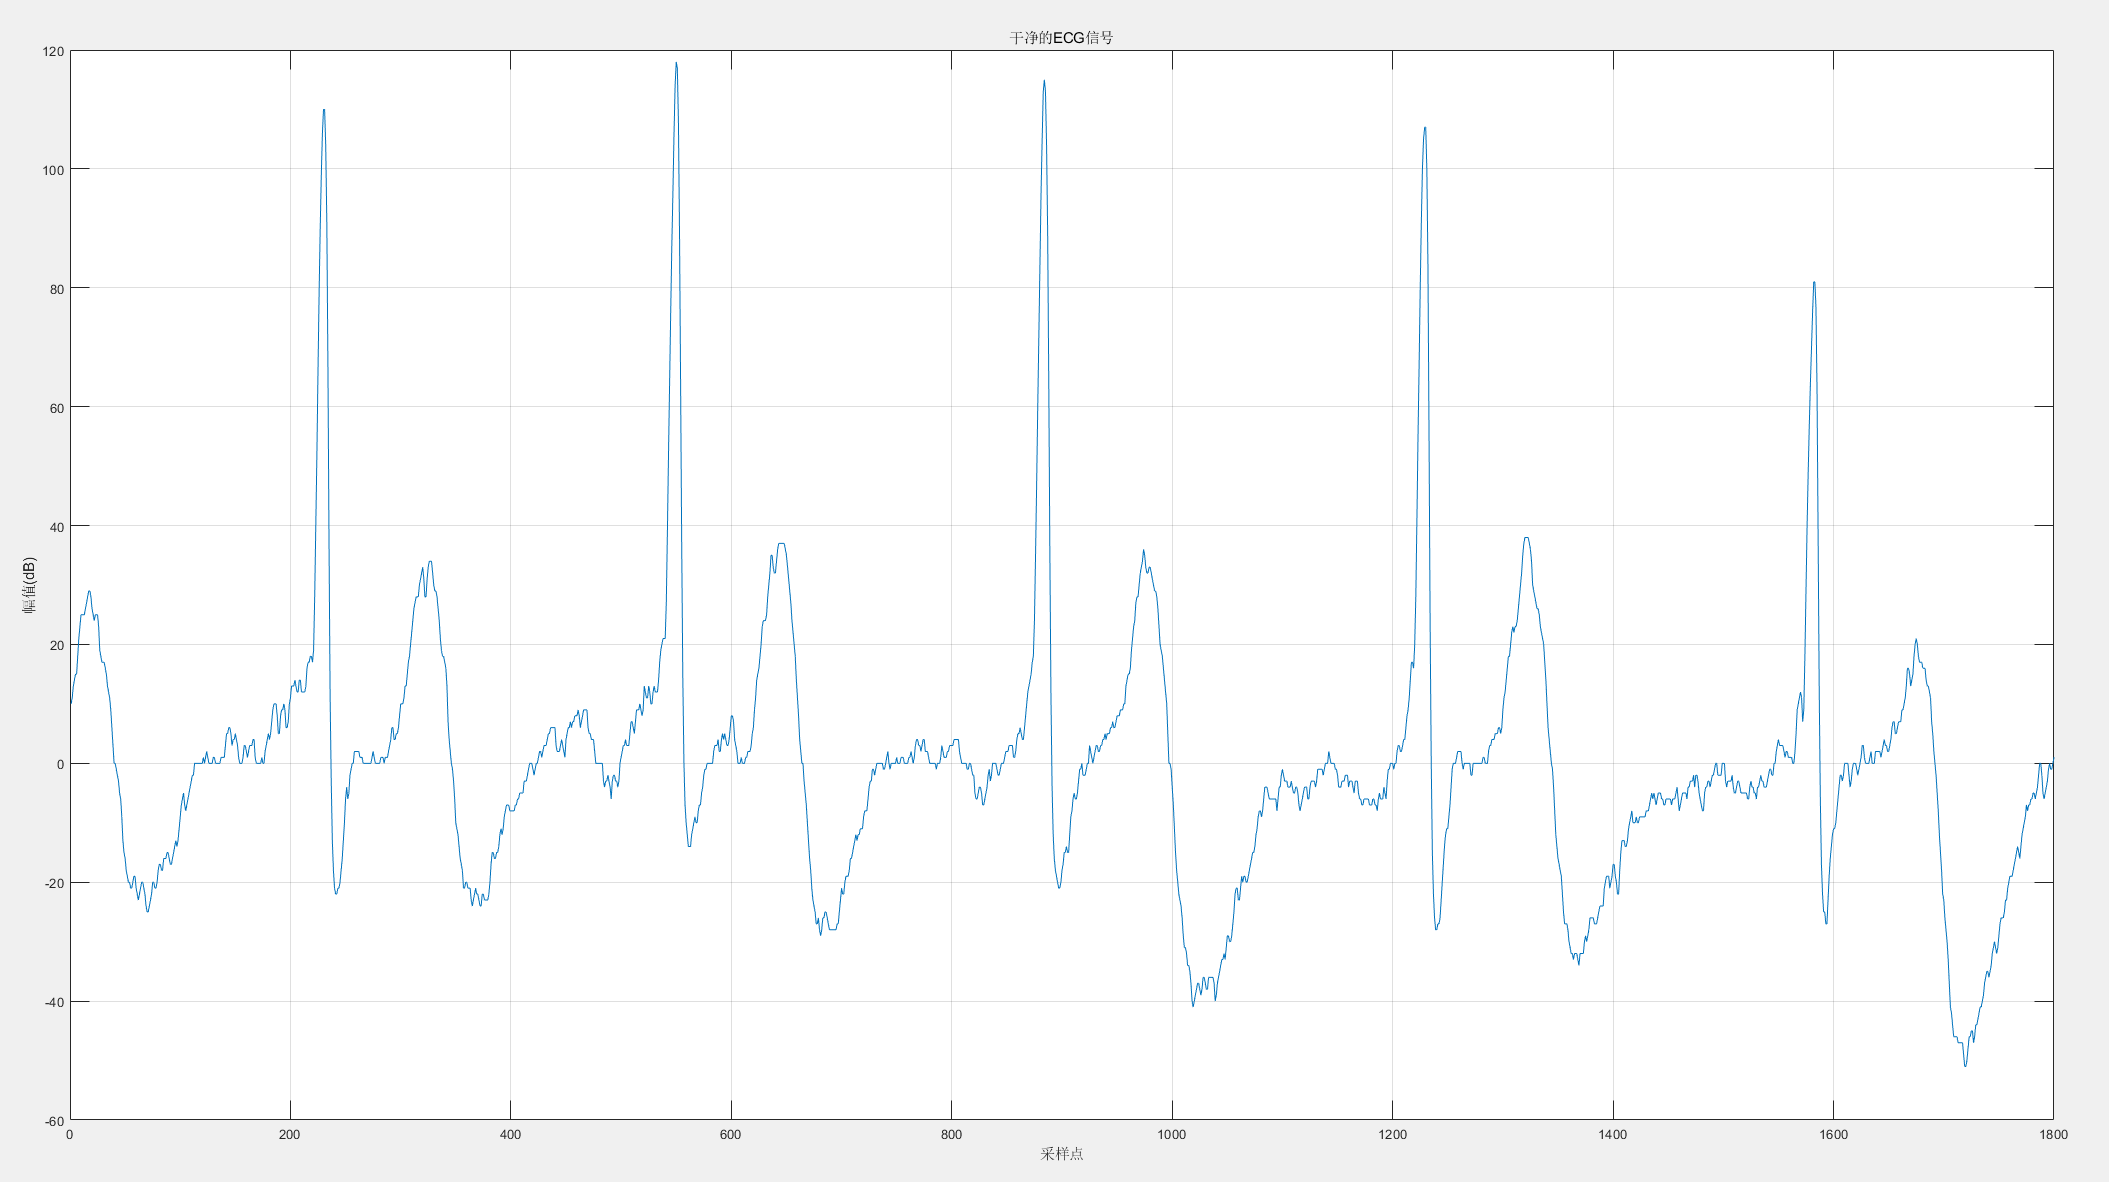
\includegraphics[width=0.9\textwidth]{figures/1.png} % 调整宽度为文本宽度的 80%
        \caption{matlab绘图} %图片标题
        \label{fig:example} % 图片标签,用于引用
\end{figure}





\subsection{题目2:数字低通滤波去除白噪音}


% 插入MATLAB代码
\begin{lstlisting}[style=matlab, caption={ MATLAB实现代码}]
% IIR和FIR低通滤波器设计与心电信号滤波实验
% 目标:设计IIR和FIR低通滤波器分别滤除心电信号中的白噪声干扰
% 滤波器指标要求:通带截止频率Wp=0.1π,阻带截止频率Ws=0.16π
%                阻带衰减不小于15dB,通带衰减不大于1dB


% 最后图像生成
%1.干净的ECG信号及其频谱
%2.含噪声的ECG信号及其频谱
%3.IIR滤波后的ECG信号及其频谱
%4.FIR滤波后的ECG信号及其频谱


clear,clc;
% 导入心电信号数据
val = importdata('Ecg.txt');
signal = val(1,1:1800);
Fs = 500; % 采样频率

% 绘制原始干净的心电信号
figure(2);
subplot(4,1,1);
plot(signal);
title('干净的ECG信号');
xlabel('采样点');ylabel('幅值(dB)');
grid on;

% 计算并绘制原始信号的频谱
XK1=fft(signal,1800); % 快速傅里叶变换
magXK1=abs(XK1); % 计算频谱幅值
figure(3);
subplot(4,1,1);
k1=0:length(magXK1)-1;
stem(k1,magXK1,'.'); % 绘制信号幅频特性曲线
xlabel('k');
ylabel('|X(k)|');
title('干净的ECG信号频谱');

% 添加高斯白噪声信号(信噪比10dB)
% 白噪声的特点是在整个频谱范围内能量均匀分布,没有特定的频率
% 它会影响信号的所有频率成分,因此需要设计低通滤波器来滤除高频噪声
signal1 = awgn(signal,10,'measured'); %10就是控制信噪比
figure(2);
subplot(4,1,2);
plot(signal1);
title('含噪声的ECG信号');
xlabel('采样点');ylabel('幅值(dB)');
grid on;

% 计算并绘制含噪声信号的频谱
XK2=fft(signal1,1800);
magXK2=abs(XK2); % 计算频谱幅值
figure(3);
subplot(4,1,2);
k2=0:length(magXK2)-1;
stem(k2,magXK2,'.'); % 绘制信号幅频特性曲线
xlabel('k');
ylabel('|X(k)|');
title('含噪声的ECG信号频谱');

% IIR低通滤波器设计(Butterworth滤波器)
% 由于白噪声分布在所有频段,而心电信号的有用成分主要集中在低频段
% 设计低通滤波器保留低频有用信号,滤除高频噪声
wp=0.1*pi;  % 通带截止频率
ws=0.16*pi; % 阻带截止频率
% 预畸变处理,将数字滤波器转换为模拟滤波器设计问题
Fp=2*Fs*tan(wp/2);
Fc=2*Fs*tan(ws/2);
Rp=1;   % 通带最大衰减(dB)
Rs=15;  % 阻带最小衰减(dB)

% 计算滤波器阶数和截止频率
[N,Wn] = buttord(Fp,Fc,Rp,Rs,'s');
% 生成Butterworth模拟原型滤波器零极点和增益
[Z,P,K] = buttap(N);
% 零极点形式转换为传递函数系数
[Bap,Aap] = zp2tf(Z,P,K);
% 低通滤波器频率变换
[b,a] = lp2lp(Bap,Aap,Wn);
% 双线性变换,将模拟滤波器转换为数字滤波器
[bz,az] = bilinear(b,a,Fs);

% 计算IIR滤波器的频率响应
[H1,W]=freqz(bz,az);
% 对含噪声信号进行IIR滤波
y1=filter(bz,az,signal1);

% 绘制IIR滤波器的幅频响应特性
figure(1);
subplot(2,1,1);
plot(W/pi,20*log10(abs(H1)));
xlabel('\omega/\pi');
ylabel('幅度 (dB)');
title('IIR低通滤波器频率响应');
grid on;

% 绘制IIR滤波后的时域信号
figure(2);
subplot(4,1,3);
plot(y1);
title('IIR滤波后的ECG信号');
xlabel('采样点');ylabel('幅值(dB)');
grid on;

% 计算并绘制IIR滤波后信号的频谱
XK3=fft(y1,1800);
magXK3=abs(XK3); % 计算频谱幅值
figure(3);
subplot(4,1,3);
k3=0:length(magXK3)-1;
stem(k3,magXK3,'.'); % 绘制信号幅频特性曲线
xlabel('k');
ylabel('|X(k)|');
title('IIR低通滤波后的ECG信号频谱');

% FIR低通滤波器设计(基于汉宁窗的FIR滤波器)
wp=0.1*pi;  % 通带截止频率
ws=0.16*pi; % 阻带截止频率
wdelta=ws-wp; % 过渡带宽度
% 根据过渡带宽度估算滤波器阶数
N=ceil(8*pi/wdelta);
wn=(wp+ws)/2; % 理想滤波器的截止频率
% 使用汉宁窗设计FIR滤波器
h=fir1(N-1,wn/pi,hanning(N));

%虽然在FIR部分没有显式指定阻带衰减,
%但通过汉宁窗设计的FIR滤波器通常可以提供大约31dB的阻带衰减,
%远大于要求的"不小于15dB"。

%使用汉宁窗设计的FIR滤波器在通带内的纹波较小,一般可以满足通带衰减"不大于1dB"的要求

% 计算FIR滤波器的频率响应
[H2,W2]=freqz(h,1,512);
% 对含噪声信号进行FIR滤波
y2=conv(signal1, h);

% 绘制FIR滤波器的幅频响应特性
figure(1);
subplot(2,1,2);
plot(W/pi,20*log10(abs(H2)));
xlabel('\omega/\pi');
ylabel('幅度 (dB)');
title('FIR低通滤波器频率响应');
grid on;

% 绘制FIR滤波后的时域信号
figure(2);
subplot(4,1,4);
plot(y2);
title('FIR滤波后的ECG信号')
xlabel('采样点');ylabel('幅值(dB)');
grid on;

% 计算并绘制FIR滤波后信号的频谱
XK4=fft(y2,1800);
magXK4=abs(XK4); % 计算频谱幅值
figure(3);
subplot(4,1,4);
k4=0:length(magXK4)-1;
stem(k4,magXK4,'.'); % 绘制信号幅频特性曲线
xlabel('k');
ylabel('|X(k)|');
title('FIR低通滤波后的ECG信号频谱');


\end{lstlisting}



\begin{figure}[H] % [H] 表示强制当前位置插入
        \centering
        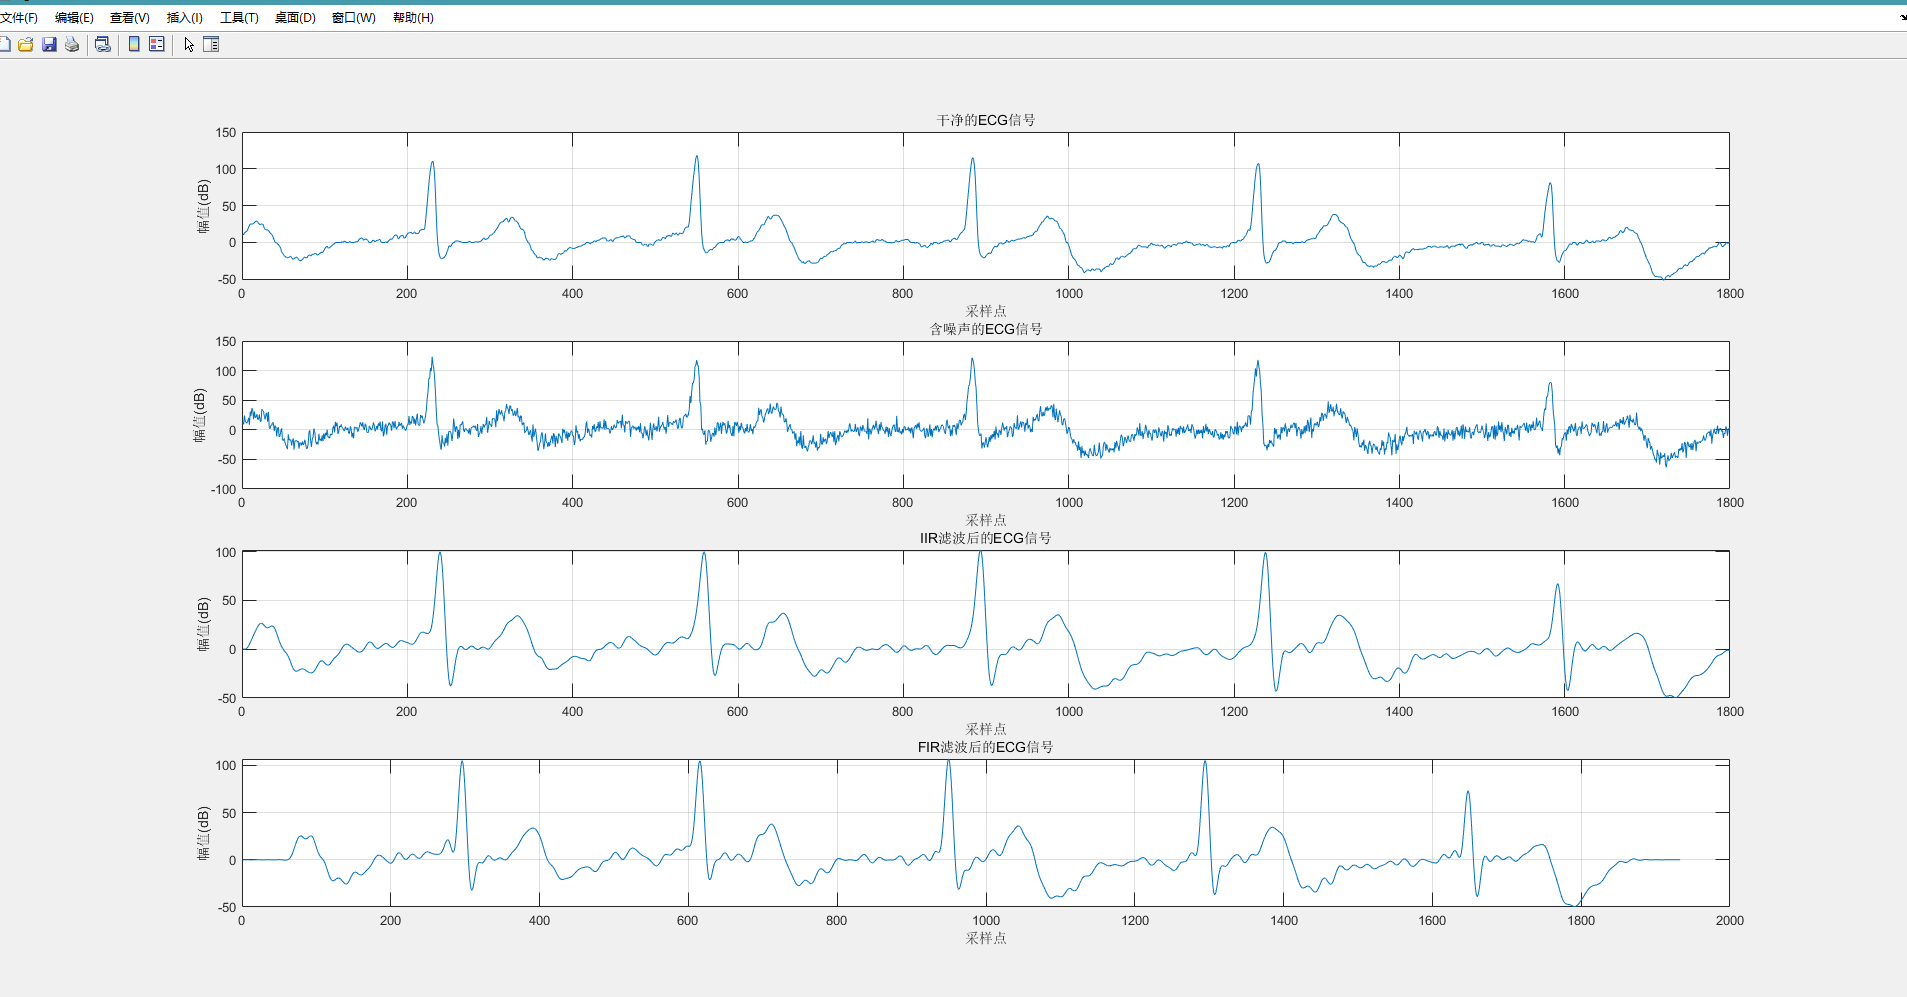
\includegraphics[width=0.9\textwidth]{figures/2_1.png} % 调整宽度为文本宽度的 80%
        \caption{matlab绘图} %图片标题
        \label{fig:example} % 图片标签,用于引用
\end{figure}

\begin{figure}[H] % [H] 表示强制当前位置插入
        \centering
        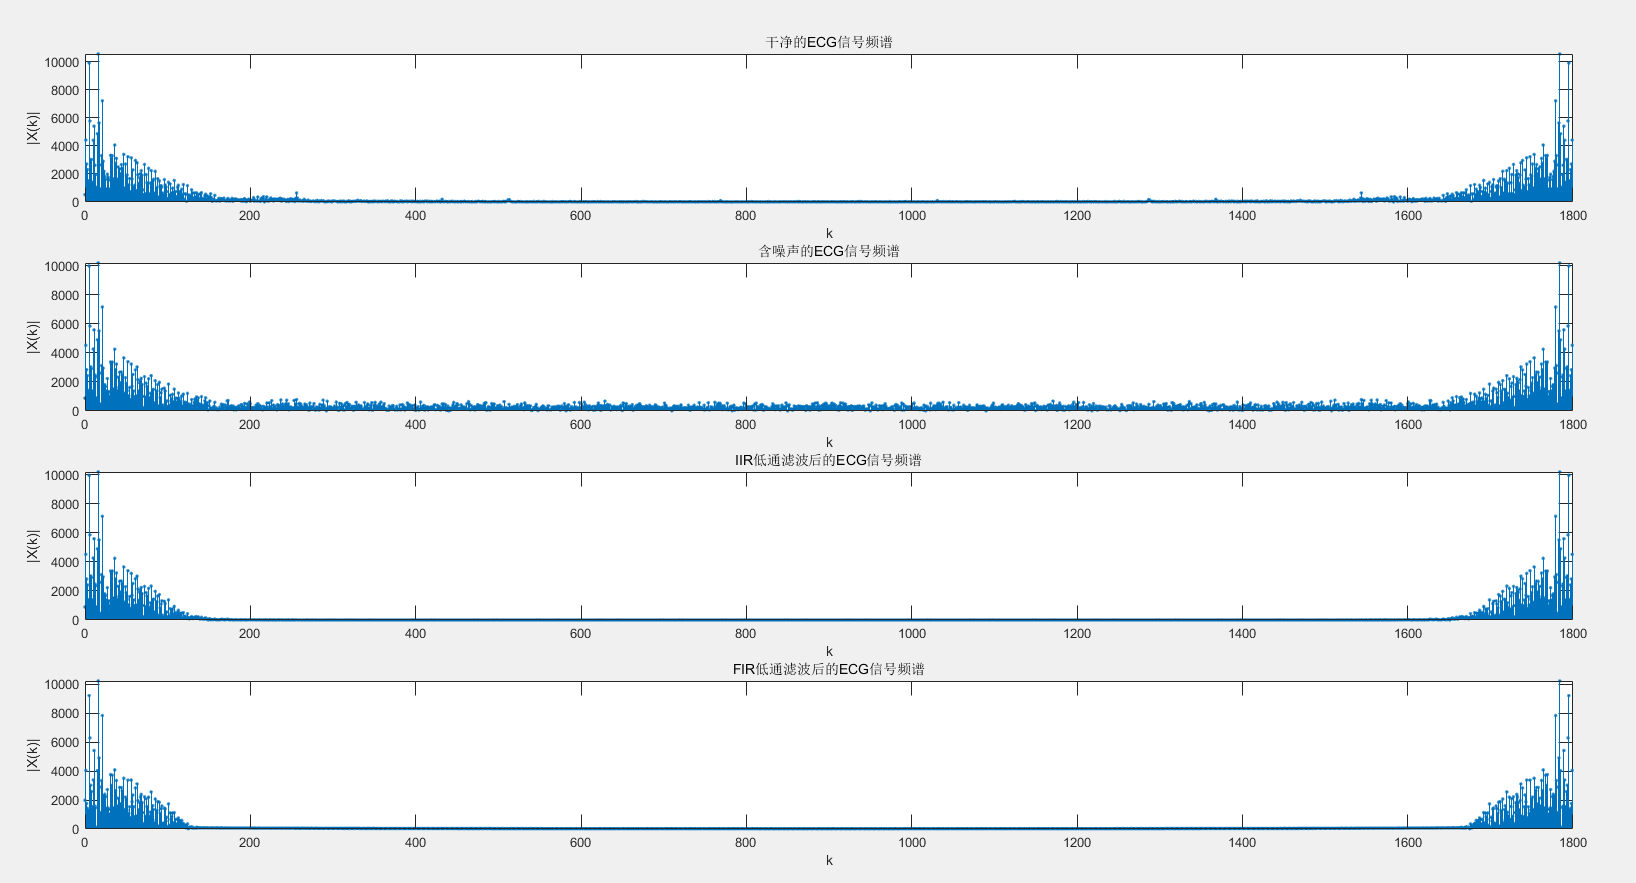
\includegraphics[width=0.9\textwidth]{figures/2_2.png} % 调整宽度为文本宽度的 80%
        \caption{matlab绘图} %图片标题
        \label{fig:example} % 图片标签,用于引用
\end{figure}

\begin{figure}[H] % [H] 表示强制当前位置插入
        \centering
        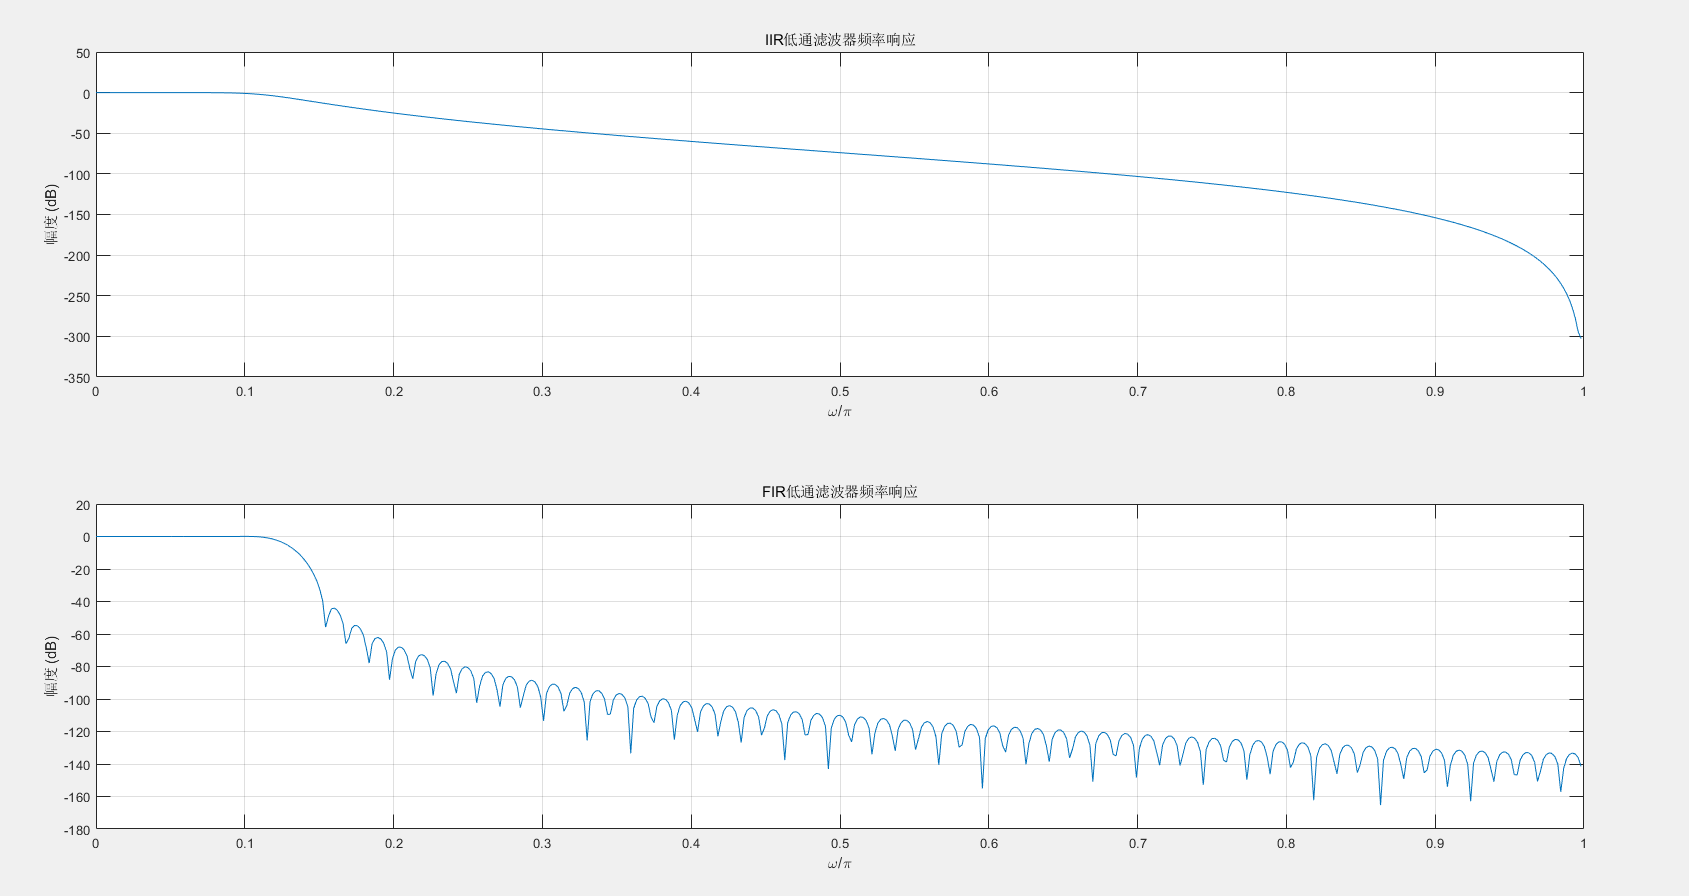
\includegraphics[width=0.9\textwidth]{figures/2_3.png} % 调整宽度为文本宽度的 80%
        \caption{matlab绘图} %图片标题
        \label{fig:example} % 图片标签,用于引用
\end{figure}


\subsection{题目3:50HZ工频IIR陷波消除}


% 插入MATLAB代码
\begin{lstlisting}[style=matlab, caption={ MATLAB实现代码}]
%50HZ工频噪声产生叠加与IIR陷波消除

clear,clc;  % 清除工作区变量和命令窗口
val = importdata('Ecg.txt');  % 导入ECG心电信号数据文件
signal = val(1,1:1800);  % 提取前1800个采样点作为处理信号
Fs = 500;  % 采样频率设置为500Hz

% 绘制原始ECG信号的时域波形
figure(2);
subplot(3,1,1);
plot(signal);
title('干净的ECG信号');
xlabel('采样点');ylabel('幅值(dB)');
grid on;

% 计算并绘制原始ECG信号的频谱
XK1=fft(signal,1800);  % 对信号进行FFT变换
magXK1=abs(XK1);  % 计算幅频特性
figure(3);
subplot(3,1,1);
k1=0:length(magXK1)-1;
stem(k1,magXK1,'.');  % 使用离散点绘制频谱
xlabel('k');
ylabel('|X(k)|');
title('干净的ECG信号频谱');

% 产生模拟工频信号(50Hz),与干净心电信号混合
av=100;
f0=50; % 工频干扰频率50Hz
t=1:length(signal);
noise2=av*cos(2*pi*f0*t/Fs);
signal2=noise2+signal; %直接相加添加工频噪声
figure(2);
subplot(3,1,2);
plot(signal2);
title('含干扰的ECG信号');
xlabel('采样点');ylabel('幅值(dB)');
grid on;
XK2=fft(signal2,1800);
magXK2=abs(XK2); %幅频特性
figure(3);
subplot(3,1,2);
k2=0:length(magXK2)-1;
stem(k2,magXK2,'.'); %信号幅频特性曲线
xlabel('k');
ylabel('|X(k)|');
title('含干扰的ECG信号频谱');

% IIR带阻滤波器设计
% 根据题目要求设置滤波器参数
% 通带下限频率 Wp1=0.18π
% 阻带下截止频率 Ws1=0.192π
% 阻带上截止频率 Ws2=0.208π
% 通带上限频率 Wp2=0.22π
% 阻带衰减不小于15dB,通带衰减不大于1dB
wp = [0.18,0.22]; % 通带边界频率
ws = [0.192,0.208]; % 阻带边界频率
Rp = 1; % 通带衰减1dB
Rs = 15; % 阻带衰减15dB
[N,Wn] = buttord(wp,ws,Rp,Rs,'s');
[b,a] = butter(N,Wn,'stop');

% 计算并绘制滤波器的频率响应曲线|H(e^jω)|
n=0:0.001:pi;
[H,W] = freqz(b,a,n);
figure(1);
subplot(1,1,1);
plot(W/pi,20*log10(abs(H)));
xlabel('\omega/\pi');
ylabel('幅度 (dB)');
title('IIR带阻滤波器频率响应');
grid on;

% 使用带阻滤波器处理含工频干扰的心电信号
[h,t]=impz(b,a);
y=conv(signal2,h); % 进行带阻滤波

% 显示滤波后的信号波形
figure(2);
subplot(3,1,3);
plot(y);
title('IIR带阻滤波后的心电信号');
xlabel('采样点');ylabel('幅值(dB)');
grid on;

% 计算并展示滤波后信号的频谱
XK3=fft(y,1800);
magXK3=abs(XK3); %幅频特性
figure(3);
subplot(3,1,3);
k3=0:length(magXK3)-1;
stem(k3,magXK3,'.'); %信号幅频特性曲线
xlabel('k');
ylabel('|X(k)|');
title('IIR带阻滤波后的信号频谱');

% 对滤波前后的心电信号的频谱进行分析比较
figure(4);
subplot(2,1,1);
plot(k2(1:900)/1800*Fs,magXK2(1:900),'b',k3(1:900)/1800*Fs,magXK3(1:900),'r');
legend('滤波前','滤波后');
title('滤波前后心电信号频谱比较');
xlabel('频率(Hz)');
ylabel('幅值');
grid on;

% 放大显示工频附近的频谱变化
subplot(2,1,2);
freq_range = [40 60]; % 工频附近频率范围
idx = round(freq_range/Fs*1800)+1;
plot(k2(idx(1):idx(2))/1800*Fs,magXK2(idx(1):idx(2)),'b',k3(idx(1):idx(2))/1800*Fs,magXK3(idx(1):idx(2)),'r');
legend('滤波前','滤波后');
title('工频(50Hz)附近频谱对比');
xlabel('频率(Hz)');
ylabel('幅值');
grid on;


\end{lstlisting}


\begin{figure}[H] % [H] 表示强制当前位置插入
        \centering
        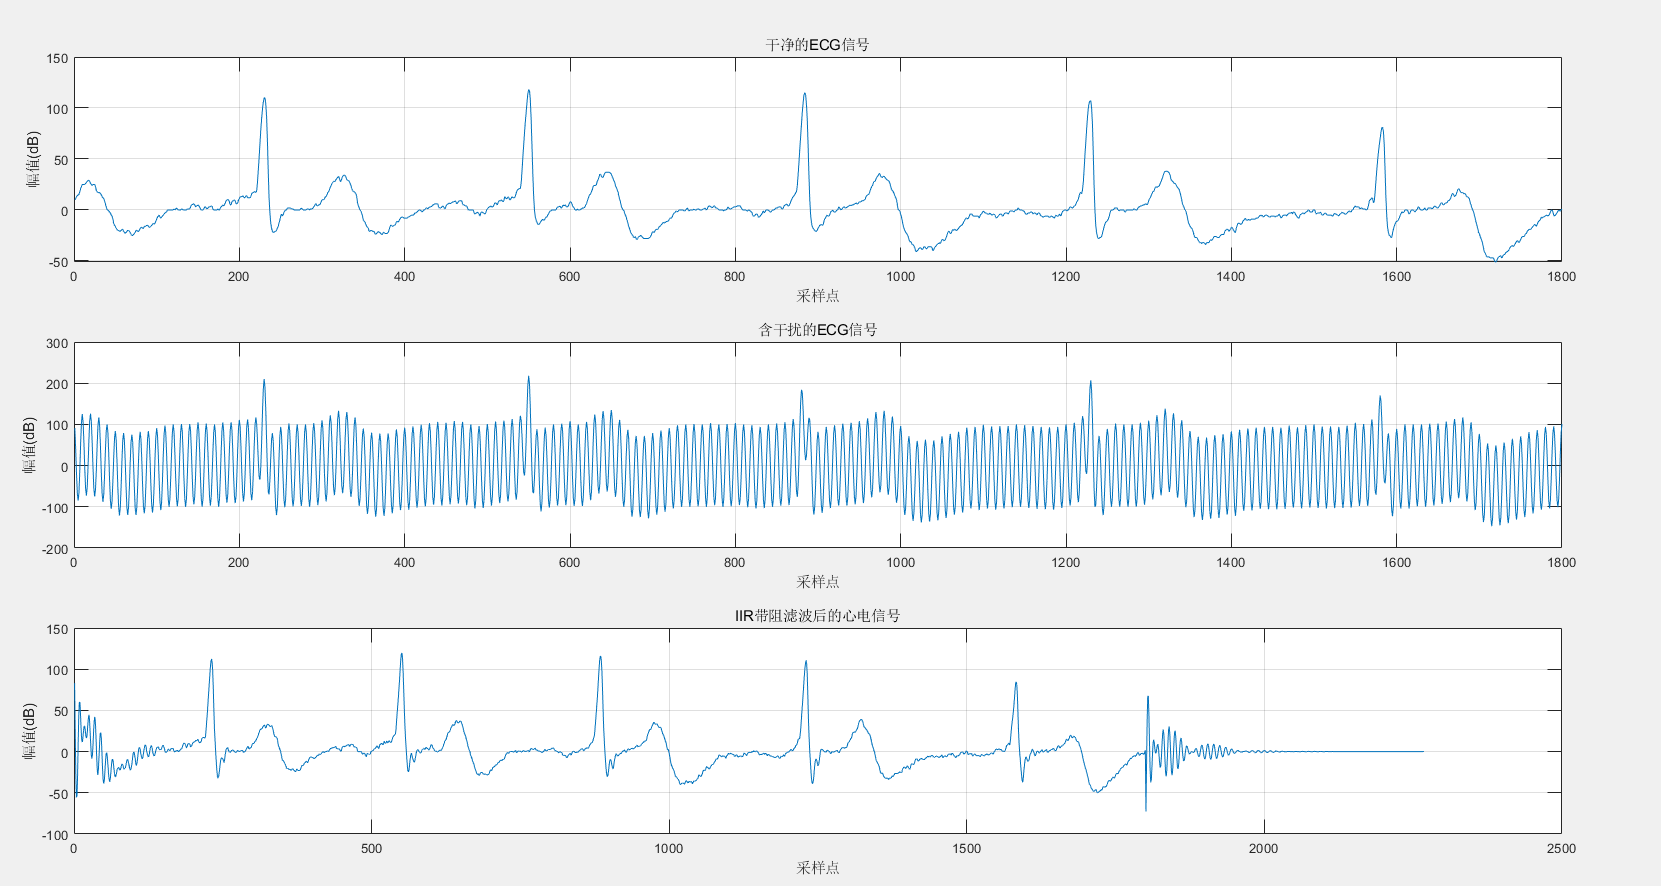
\includegraphics[width=0.9\textwidth]{figures/3_1.png} % 调整宽度为文本宽度的 80%
        \caption{IIR带阻滤波器频率响应} %图片标题
        \label{fig:3_1} % 图片标签,用于引用
\end{figure}

\begin{figure}[H] % [H] 表示强制当前位置插入
        \centering
        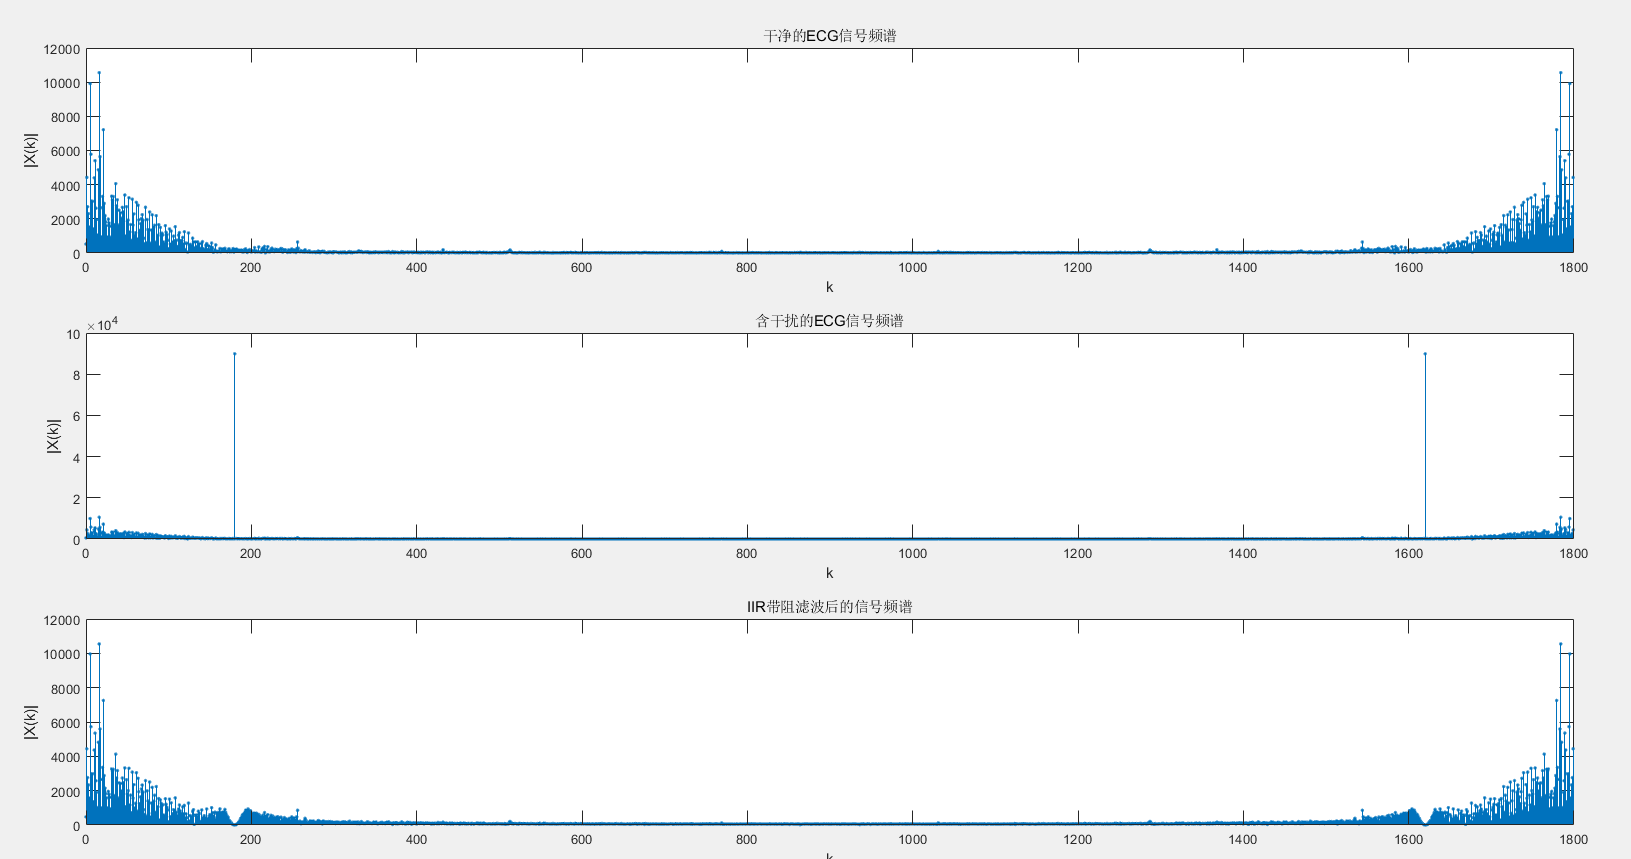
\includegraphics[width=0.9\textwidth]{figures/3_2.png} % 调整宽度为文本宽度的 80%
        \caption{心电信号的时域波形} %图片标题
        \label{fig:3_2} % 图片标签,用于引用
\end{figure}

\begin{figure}[H] % [H] 表示强制当前位置插入
        \centering
        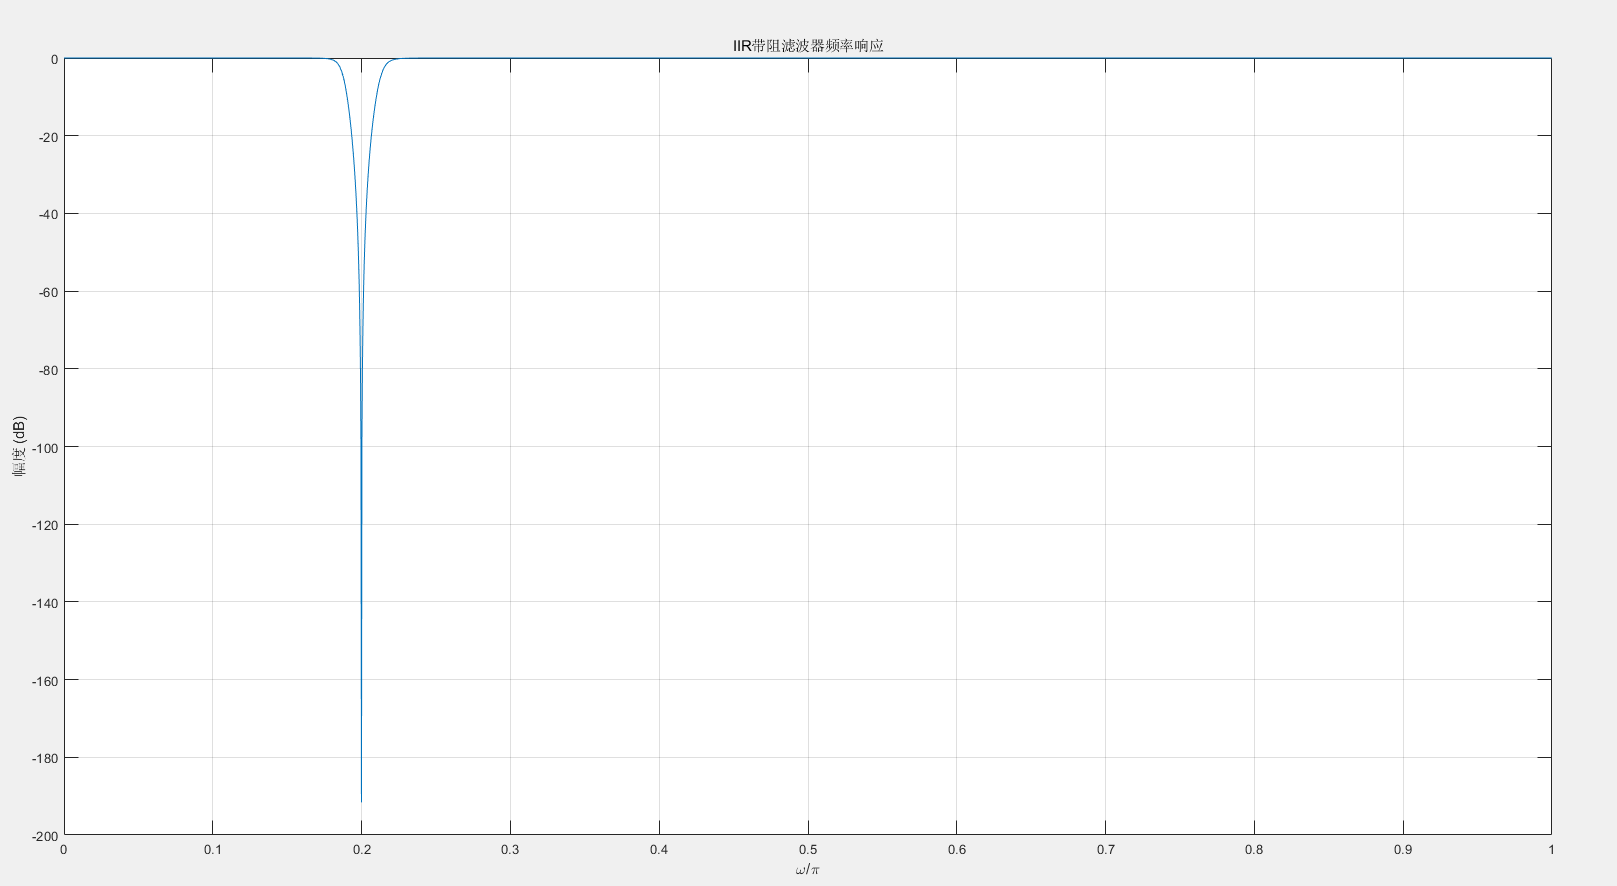
\includegraphics[width=0.9\textwidth]{figures/3_3.png} % 调整宽度为文本宽度的 80%
        \caption{心电信号的频谱分析} %图片标题
        \label{fig:3_3} % 图片标签,用于引用
\end{figure}

\begin{figure}[H] % [H] 表示强制当前位置插入
        \centering
        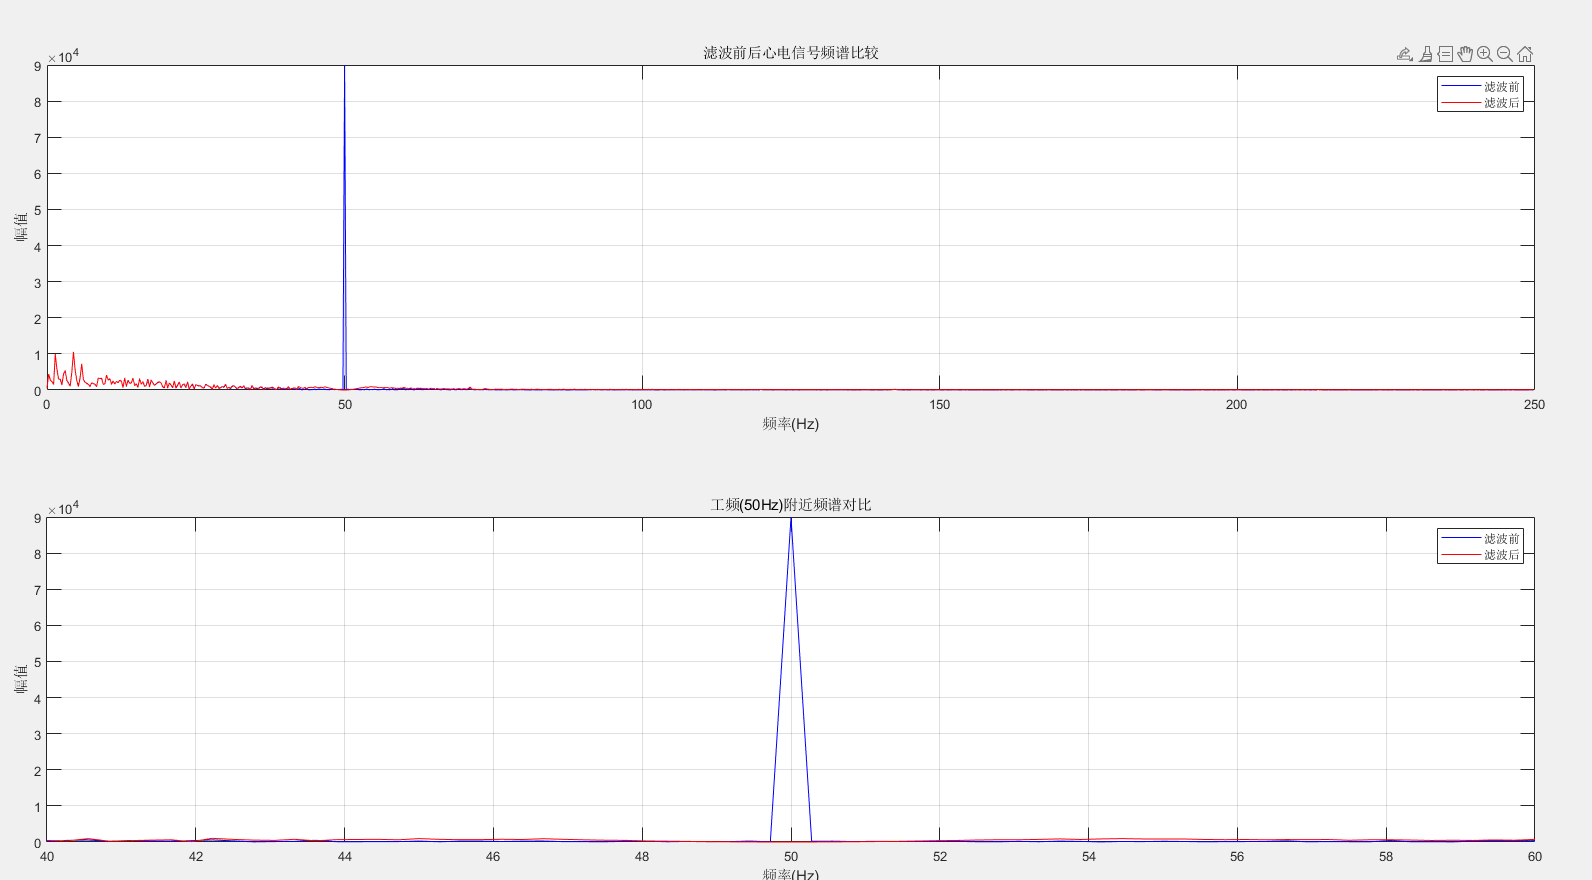
\includegraphics[width=0.9\textwidth]{figures/3_4.png} % 调整宽度为文本宽度的 80%
        \caption{滤波前后频谱对比} %图片标题
        \label{fig:3_4} % 图片标签,用于引用
\end{figure}


\subsection{题目4:高通滤波器消除基线漂移}

% 插入MATLAB代码
\begin{lstlisting}[style=matlab, caption={高通滤波器设计与实现}]
%高通滤波器消除基线漂移

clear,clc;
% 导入心电信号数据
val = importdata('Ecg.txt');
signal = val(1,1:1800);
Fs = 500; % 采样频率

% 绘制原始干净的心电信号
figure(2);
subplot(3,1,1);
plot(signal);
title('干净的ECG信号');
xlabel('采样点');ylabel('幅值(dB)');
grid on;

% 计算并绘制原始信号的频谱
XK1=fft(signal,1800); % 快速傅里叶变换
magXK1=abs(XK1); % 计算频谱幅值
figure(3);
subplot(3,1,1);
k1=0:length(magXK1)-1;
stem(k1,magXK1,'.'); % 绘制信号幅频特性曲线
xlabel('k');
ylabel('|X(k)|');
title('干净的ECG信号频谱');

% 产生模拟基线漂移信号(低频漂移,频率一般低于0.5Hz)
% 使用正弦波来模拟基线漂移
t = 1:length(signal);
% 创建低频的正弦波,频率为0.3Hz,振幅较大以明显展示效果
baseline_wander = 100*sin(2*pi*0.3*t/Fs);
% 将基线漂移添加到原始信号
signal_with_baseline = signal + baseline_wander;

% 绘制带有基线漂移的心电信号
figure(2);
subplot(3,1,2);
plot(signal_with_baseline);
title('带有基线漂移的ECG信号');
xlabel('采样点');ylabel('幅值(dB)');
grid on;

% 计算并绘制带基线漂移信号的频谱
XK2=fft(signal_with_baseline,1800);
magXK2=abs(XK2); % 计算频谱幅值
figure(3);
subplot(3,1,2);
k2=0:length(magXK2)-1;
stem(k2,magXK2,'.'); % 绘制信号幅频特性曲线
xlabel('k');
ylabel('|X(k)|');
title('带基线漂移的ECG信号频谱');

% 设计IIR高通滤波器
% 根据题目要求,通带截止频率为0.0028π rad/sample,对应约0.7Hz
% 通带衰减不大于1dB,阻带衰减不小于15dB
wp = 0.0028*pi; % 通带截止频率 
ws = 0.0014*pi; % 阻带截止频率(设为通带截止频率的一半)
Rp = 1;   % 通带最大衰减(dB)
Rs = 15;  % 阻带最小衰减(dB)

% 使用butter设计巴特沃斯高通滤波器
[n, wn] = buttord(wp/pi, ws/pi, Rp, Rs); % 计算滤波器阶数
[b, a] = butter(n, wn, 'high'); % 设计高通滤波器

% 计算并绘制滤波器的频率响应
[H, W] = freqz(b, a, 1024);
figure(1);
plot(W/pi, 20*log10(abs(H)));
xlabel('\omega/\pi');
ylabel('幅度 (dB)');
title('IIR高通滤波器频率响应');
grid on;

% 应用滤波器处理含基线漂移的信号
filtered_signal = filtfilt(b, a, signal_with_baseline); % 使用零相位滤波

% 绘制滤波后的信号
figure(2);
subplot(3,1,3);
plot(filtered_signal);
title('高通滤波后的ECG信号');
xlabel('采样点');ylabel('幅值(dB)');
grid on;

% 计算并绘制滤波后信号的频谱
XK3=fft(filtered_signal,1800);
magXK3=abs(XK3); % 计算频谱幅值
figure(3);
subplot(3,1,3);
k3=0:length(magXK3)-1;
stem(k3,magXK3,'.'); % 绘制信号幅频特性曲线
xlabel('k');
ylabel('|X(k)|');
title('高通滤波后的ECG信号频谱');

% 对比滤波前后的信号频谱变化,特别关注低频部分
figure(4);
subplot(2,1,1);
% 显示完整频谱比较
plot(k2(1:900)/1800*Fs, magXK2(1:900), 'b', k3(1:900)/1800*Fs, magXK3(1:900), 'r');
legend('滤波前','滤波后');
title('滤波前后心电信号频谱比较');
xlabel('频率(Hz)');
ylabel('幅值');
grid on;

% 放大显示低频部分的频谱变化
subplot(2,1,2);
freq_range = [0 2]; % 低频范围,关注基线漂移
idx = round(freq_range/Fs*1800)+1;
plot(k2(idx(1):idx(2))/1800*Fs, magXK2(idx(1):idx(2)), 'b', ...
     k3(idx(1):idx(2))/1800*Fs, magXK3(idx(1):idx(2)), 'r');
legend('滤波前','滤波后');
title('低频(0-2Hz)部分频谱对比');
xlabel('频率(Hz)');
ylabel('幅值');
grid on;
\end{lstlisting}

\begin{figure}[H] % [H] 表示强制当前位置插入
        \centering
        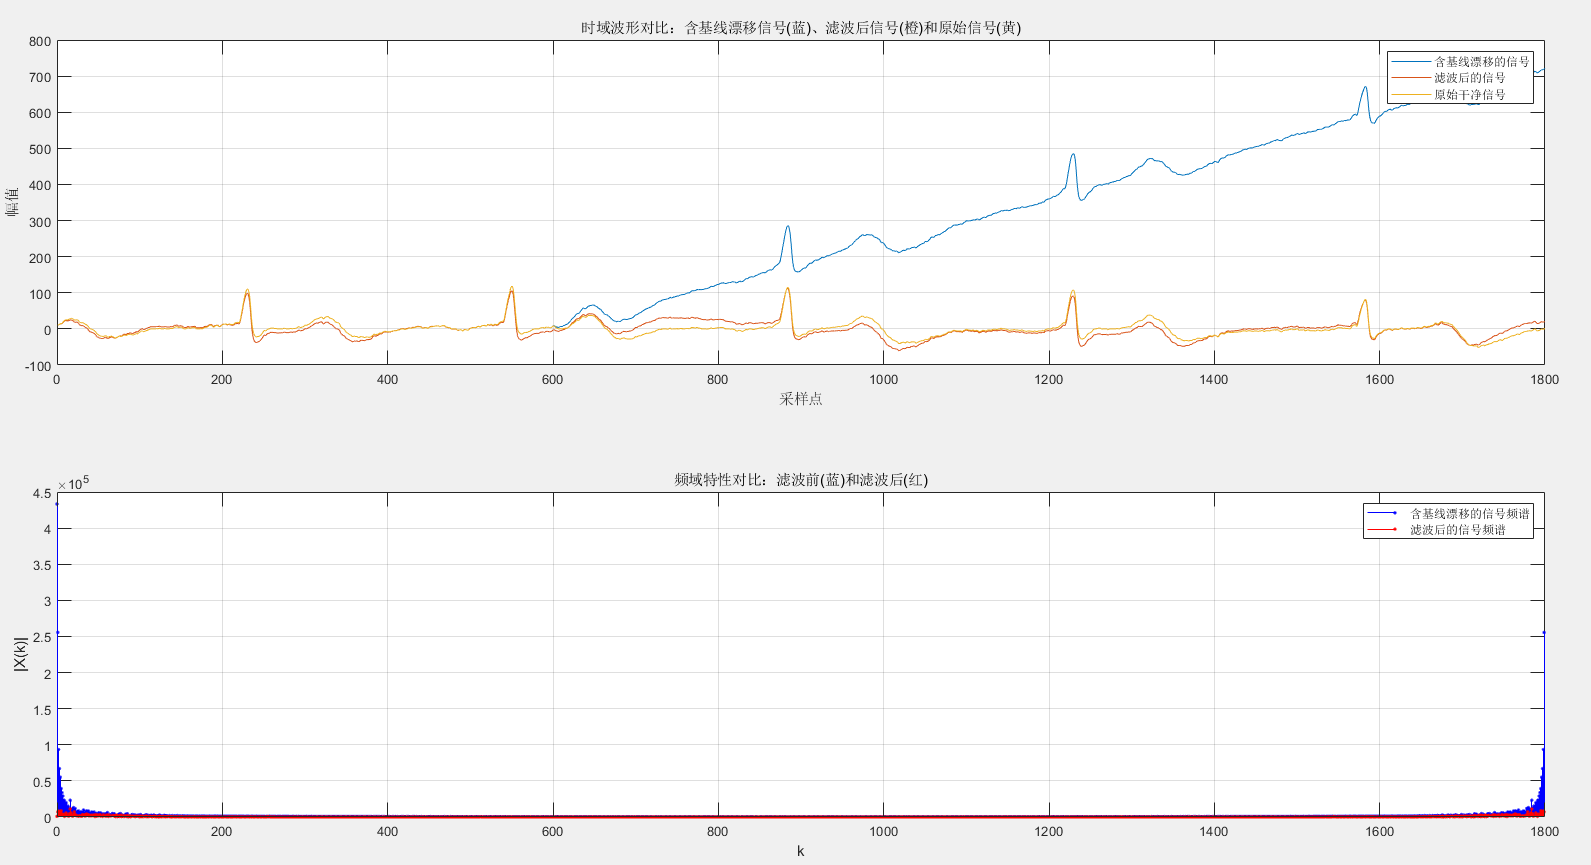
\includegraphics[width=0.9\textwidth]{figures/4_1.png} % 调整宽度为文本宽度的 80%
        \caption{IIR高通滤波器频率响应} %图片标题
        \label{fig:4_1} % 图片标签,用于引用
\end{figure}

\begin{figure}[H] % [H] 表示强制当前位置插入
        \centering
        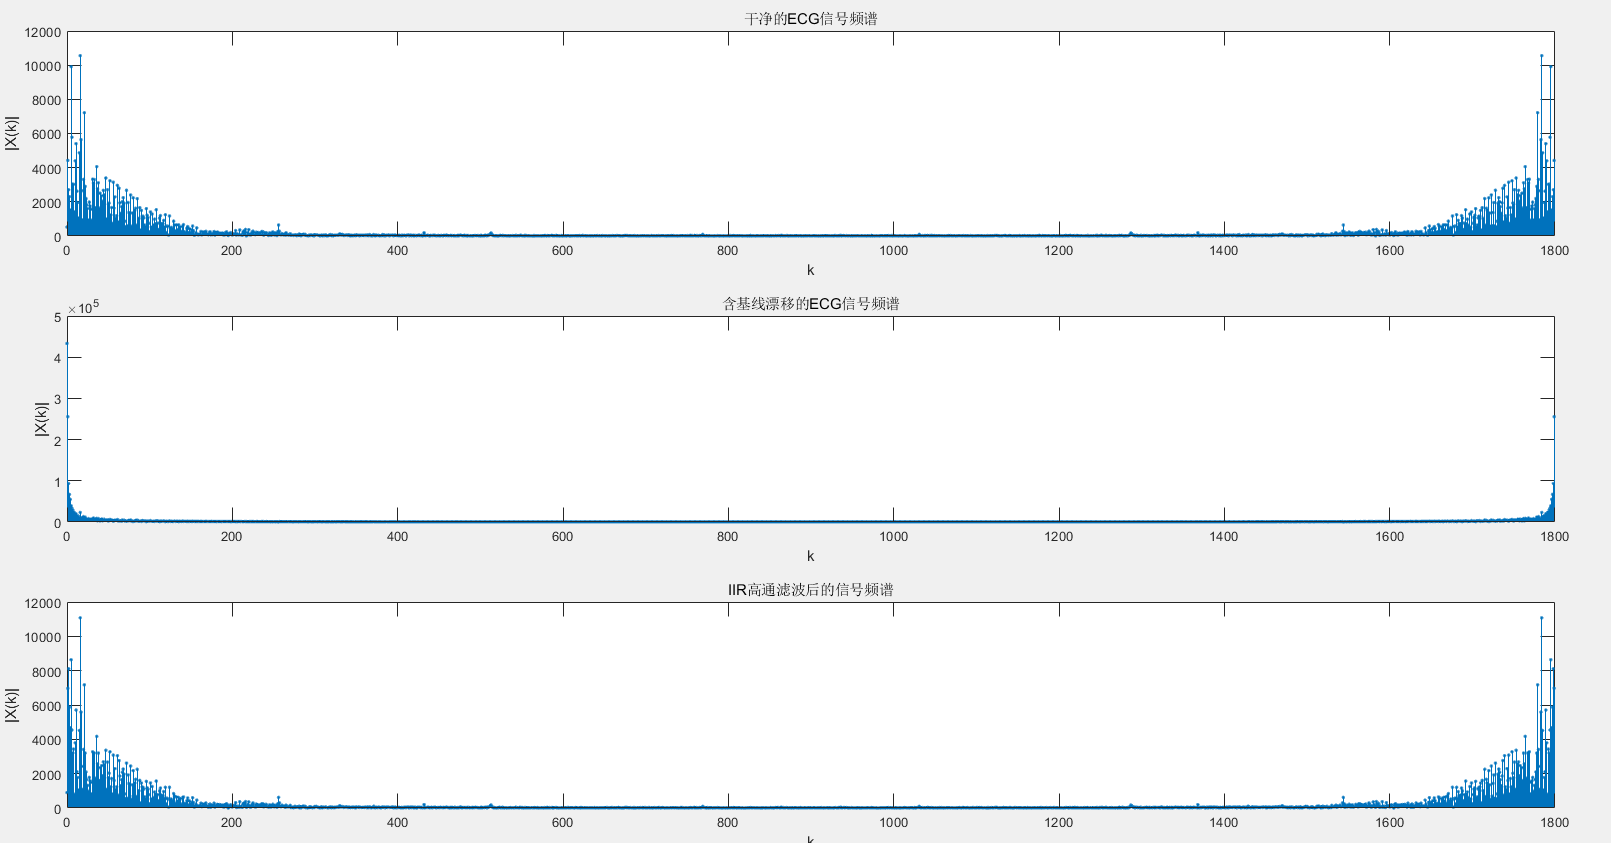
\includegraphics[width=0.9\textwidth]{figures/4_2.png} % 调整宽度为文本宽度的 80%
        \caption{基线漂移处理前后的时域波形} %图片标题
        \label{fig:4_2} % 图片标签,用于引用
\end{figure}

\begin{figure}[H] % [H] 表示强制当前位置插入
        \centering
        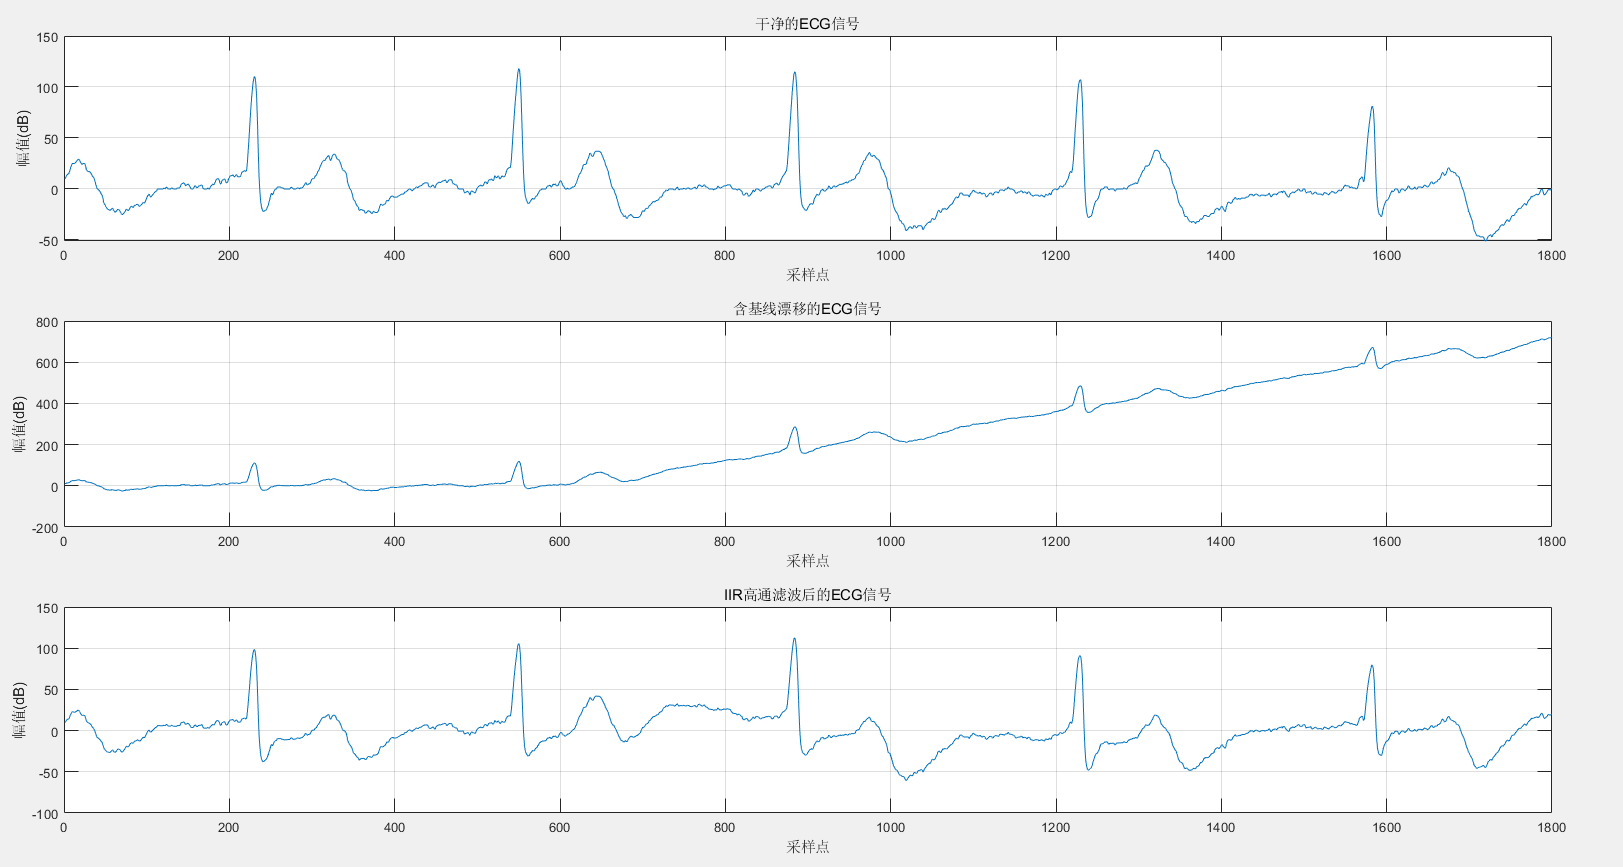
\includegraphics[width=0.9\textwidth]{figures/4_3.png} % 调整宽度为文本宽度的 80%
        \caption{基线漂移处理前后的频谱} %图片标题
        \label{fig:4_3} % 图片标签,用于引用
\end{figure}

\begin{figure}[H] % [H] 表示强制当前位置插入
        \centering
        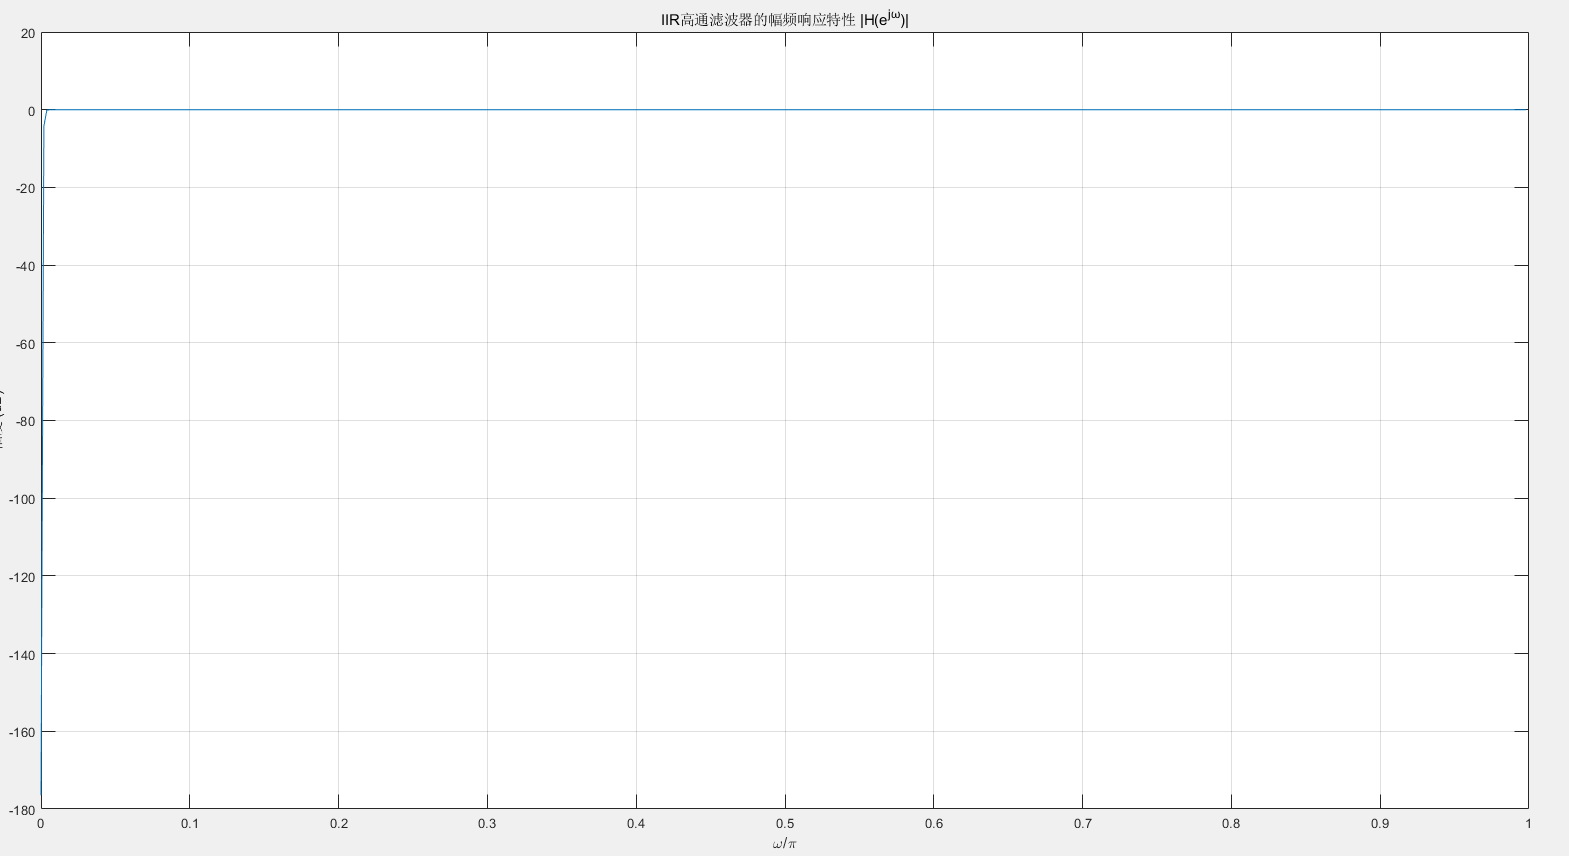
\includegraphics[width=0.9\textwidth]{figures/4_4.png} % 调整宽度为文本宽度的 80%
        \caption{低频部分频谱对比} %图片标题
        \label{fig:4_4} % 图片标签,用于引用
\end{figure}

\section{实验小结}

本实验通过四个题目,系统地探究了数字信号处理技术在心电信号处理中的应用。主要收获如下:

\subsection{数字滤波器设计与应用}

\begin{enumerate}
    \item \textbf{IIR与FIR滤波器对比}:实验证明IIR滤波器可以用较低阶数实现较陡峭的频率响应,计算效率高;而FIR滤波器虽然阶数较高,但具有严格的线性相位特性,能更好地保持心电信号波形不失真。
    
    \item \textbf{滤波器选择与参数设计}:针对不同类型的干扰,选择合适的滤波器类型至关重要。对于白噪声使用低通滤波器,对于工频干扰使用带阻滤波器,对于基线漂移使用高通滤波器。
    
    \item \textbf{频域分析的重要性}:通过频谱分析可以清晰地观察到干扰信号的特征及滤波效果,帮助优化滤波器设计参数。
\end{enumerate}

\subsection{心电信号处理的实践经验}

\begin{enumerate}
    \item \textbf{干扰识别与处理}:成功识别并处理了三种典型干扰:白噪声、工频干扰和基线漂移,掌握了针对性处理方法。
    
    \item \textbf{信号质量评估}:通过时域波形和频域分析相结合的方式,可以全面评估滤波效果,确保处理后的信号保留了关键的诊断信息。
    
    \item \textbf{滤波器串联应用}:在实际应用中,可能需要多种滤波器串联使用,以处理复杂的混合干扰。
\end{enumerate}

\subsection{工程实践意义}

本实验的方法和结果对生物医学信号处理具有重要的实践意义,特别是在可穿戴医疗设备和远程医疗监测系统中,高质量的心电信号处理对准确诊断至关重要。实验中掌握的数字滤波技术为后续开发更复杂的信号处理算法奠定了基础。

总之,通过本次实验,我们不仅掌握了数字滤波器设计和应用的基本技能,还深入理解了心电信号的特性及其处理方法,这对未来在医学信号处理领域的进一步学习和研究具有重要的指导意义。

\end{document}